\documentclass[Deriaz_Traiber_Labo02.tex]{subfiles}


\begin{document}
\chapter{Introduction}
L'objectif de ce laboratoire est de réaliser 4 antennes :
\begin{itemize}
\item Dipôle sur FR-4
\item Dipôle sur céramique
\item Patch sur FR-4
\item Patch sur céramique
\end{itemize}
\begin{figure}[H]
\centering
\begin{subfigure}{0.5\textwidth}
\centering
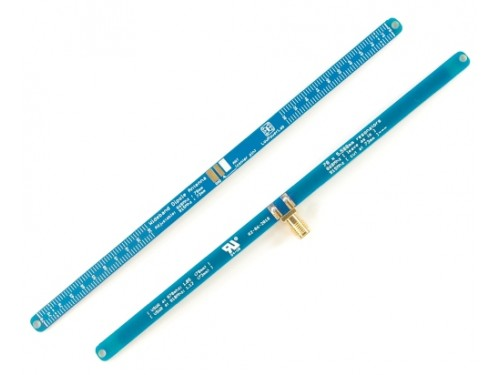
\includegraphics[width=6cm]{Figure/antenne_dipole.jpg}
\caption[caption]{Antenne dipôle\footnotemark}
\end{subfigure}
\begin{subfigure}{0.5\textwidth}
\centering
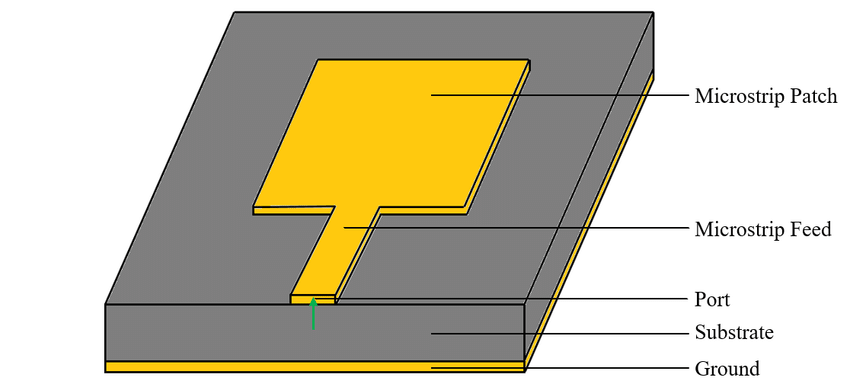
\includegraphics[width=8cm]{Figure/antenne_patch.png}
\caption[caption]{Antenne patch\footnotemark}
\end{subfigure}
\end{figure}

\footnotetext[1]{\url{https://lowpowerlab.com/shop/image/cache/data/Antennas/DSC_2424_500-500x375.jpg}}
\footnotetext[2]{\url{https://www.researchgate.net/profile/Mehdi-Chowdhury-3/publication/330277091/figure/fig1/AS:741744744337408@1553857136077/Basic-Structure-of-a-microstrip-patch-antenna-8.ppm}}

Chaque antenne sera réalisée et simulée dans le logiciel CST. Les paramètres de bases seront donnés ou calculés puis, par itérations successives, seront ajustés pour adapter les antennes (fréquence(s) de résonance et bande passante). Le but est de comprendre et de pouvoir décrire le rôle de chaque paramètre sur les caractéristiques de l'antenne